\documentclass[10pt]{beamer}

%% Chinese support
%% \usepackage[adobefonts,nocap]{ctex}

%% Fonts
\usepackage{multicol}
\usepackage{mathabx}
\usepackage[scaled]{helvet}
\usepackage{lmodern}
\usepackage{eulervm}
\usefonttheme[onlymath]{serif}
\usefonttheme{professionalfonts}
\usefonttheme{structurebold}
\usepackage{bm}
\usepackage{verbatim}

%% Color & Theme
\definecolor{SUblue}{RGB}{0,0,180}
\usecolortheme[RGB={0,0,180}]{structure}
\usetheme{Boadilla}
\setbeamertemplate{navigation symbols}{}
\setbeamertemplate{itemize items}[circle]
\setbeamertemplate{enumerate items}[circle]
\setbeamerfont{title}{size=\large}
\setbeamerfont{frametitle}{size=\large}
\setbeamerfont{framesubtitle}{size=\large,shape =$\color{violet}{\looparrowdownright}~$}
\setbeamercolor{title}{fg=white, bg= SUblue!75!green}
\setbeamercolor{framesubtitle}{fg=violet}
%\setlength{\leftmargini}{5pt}


\title[Statistical Computing]{{\textbf{Computational Linear Algebra}}}

\author[Feng Li]{\includegraphics[height=2cm]{cufelogo}\\
  \vspace{0.5cm}\textbf{Feng Li\\\texttt{feng.li@cufe.edu.cn}}}

\institute[SAM.CUFE.EDU.CN]{\footnotesize{\textbf{School of
      Statistics and Mathematics\\ Central University of Finance and
      Economics}}}
\date{}

%%%%%%%%%%%%%%%%%%%%%%%%%%%%%%%%%%%%%%%%%%%%%%%%%%%%%%%%%%%%%%%%%%%%%%
\begin{document}

%% Title page
\begin{frame}[plain]
  \titlepage
  \tiny{Revised on \today}
\end{frame}


%% Outline page
\section*{Today we are going to learn...}
\begin{frame}
  \frametitle{Today we are going to learn...}
  \tableofcontents
\end{frame}

\section{Basic linear algebra}

\begin{frame}
  \frametitle{The determinant of a matrix}
  \begin{itemize}
  \item The definition of a matrix determinant
    \begin{equation*}
      \det(A) = \sum_{\sigma \in S_n} sgn(\sigma) \prod_{i=1}^n a_{i,\sigma(i)}
    \end{equation*}

  \item The calculation becomes more complicated. It can be found in R
    using the \texttt{det()} function.

  \item The \texttt{determinant()} function can calculate the log determinant.

  \item Verify the following properties

    \begin{itemize}
    \item $\det(A^{\rm T}) = \det(A)$
    \item $\det(A^{-1}) = \frac{1}{\det(A)}=\det(A)^{-1}$
    \item For square matrices A and B of equal size,
      $\det(AB) = \det(A)\det(B)$.
    \item $\det(cA) = c^n\det(A)$ for an $n \times n$ matrix.

    \end{itemize}

  \end{itemize}
\end{frame}


\begin{frame}
  \frametitle{Eigenvalues and eigenvectors}

  \begin{itemize}
  \item An eigenvector of a square matrix A is a non-zero vector v
    that, when the matrix is multiplied by v, yields a constant
    multiple of v, the multiplier being commonly denoted by
    $\lambda$. That is: $A v = \lambda v$.

  \item If A is also positive-definite, positive-semidefinite,
    negative-definite, or negative-semidefinite every eigenvalue is
    positive, non-negative, negative, or non-positive respectively.

  \item Eigenvalues and eigenvectors can be computed using the
    function \texttt{eigen()}

  \item Eigenvalues can be used to check if a matrix is invertible.

  \item The determinant of A is the product of all eigenvalues:
    $\operatorname{det}(A) = \prod_{i=1}^n \lambda_i=\lambda_1\lambda_2\cdots\lambda_n$

  \item
    The trace of A, defined as the sum of its diagonal elements, is also the sum of all eigenvalues:
    $\operatorname{tr}(A) = \sum_{i=1}^n A_{i i} = \sum_{i=1}^n \lambda_i = \lambda_1+ \lambda_2 +\cdots+ \lambda_n$

  \end{itemize}

\end{frame}

\begin{frame}
  \frametitle{Triangular matrices}

  \begin{itemize}
  \item The functions \texttt{lower.tri()} and \texttt{upper.tri()}
    can be used to obtain the lower and upper triangular parts of
    matrices.
  \end{itemize}
\end{frame}

\begin{frame}[fragile]
  \frametitle{Outer Products}

  \begin{itemize}
  \item The function \texttt{outer()} is sometimes useful in
    statistical calculations. It can be used to perform an operation
    on all possible pairs of elements coming from two vectors.

  \item Example

\begin{verbatim}
> x1 <- seq(1, 5)
> outer(x1, x1, "/")
> y <- seq(5, 10)
> outer(x1, y, "+")
\end{verbatim}

  \end{itemize}
\end{frame}


\begin{frame}
  \frametitle{Kronecker product}

  \begin{itemize}
  \item If $A$ is an $m\times n$ matrix and $B$ is a $p \times q$
    matrix, then the Kronecker product $A \otimes  B$ is the $mp \times nq$ block matrix:
    \begin{equation*}
          \mathbf{A}\otimes\mathbf{B} = \begin{bmatrix} a_{11} \mathbf{B} & \cdots & a_{1n}\mathbf{B} \\ \vdots & \ddots & \vdots \\ a_{m1} \mathbf{B} & \cdots & a_{mn} \mathbf{B} \end{bmatrix}
    \end{equation*}

  \item The function \texttt{kronecker()} can be used to compute the Kronecker product
of two matrices and other more general products.

  \end{itemize}

\end{frame}

\section{QR Decomposition}

\begin{frame}
  \frametitle{The matrix inverse}

  \begin{itemize}
  \item The usual definition of \texttt{square matrix inverse} is $A^{-1}A =
    AA^{-1}=I$ which is not commonly used in practice. The solution is
    \textbf{unique} when $A$ is not singular.

  \item \textbf{The general inverse} for $A_{m\times n}$

    \begin{itemize}
    \item The definition: $A^{+} A = I$

    \item Notice that $(A'A)^{-1}A'A=I$, the above definition actually
      means $A^{+}=(A'A)^{-1}A'$.

    \item The general inverse in \textbf{not unique} but useful.

    \end{itemize}

  \end{itemize}

\end{frame}


\begin{frame}
  \frametitle{QR decomposition}

  \begin{itemize}
  \item QR decomposition is a decomposition of a matrix $A$ into a
    product $A = QR$ of an orthogonal matrix $Q$ and an upper
    triangular matrix $R$.

  \item Compared to the direct matrix inverse, inverse solutions using
    QR decomposition are more numerically stable as evidenced by their
    reduced condition numbers.


  \item To solve the underdetermined ($m < n$ ) linear problem $Ax=b$
    where the matrix $A$ has dimensions $m \times n$ and rank $m$

    \begin{itemize}
    \item first find the QR factorization of the transpose of $A$:
      $A^T=QR$ , where $Q$ is an orthogonal matrix
      (i.e. $Q^T=Q^{-1}$), and $R$ has a special form:
      $R=\begin{bmatrix} R_1 \\ 0\end{bmatrix}$. Here $R_1$ is a
      square $m \times m$ right triangular matrix, and the zero matrix
      has dimension $(n-m) \times m$.

    \item it can be shown that a solution to the inverse problem can
      be expressed as: $x = Q \begin{bmatrix} (R_1^T)^{-1}b \\
        0 \end{bmatrix} = [Q_1,Q_2] \begin{bmatrix} (R_1^T)^{-1}b \\
        0 \end{bmatrix} = Q_1(R_1^T)^{-1}b$

    \end{itemize}

  \end{itemize}

\end{frame}


\begin{frame}
  \frametitle{The linear model with QR}

  \begin{itemize}
  \item For a linear model $y=X\hat\beta$, the QR approach is slightly
    slower than $(X'X)^{-1}Xy$ but more accurate.

  \item The procedure is to compute the \textbf{QR decomposition} of
    $X$ to get $R$ and $Q'Y$ , solve $R\beta = Q'y$.


    \begin{itemize}
    \item As $X=QR$, the linear regression is now written As
      \begin{equation*}
        \hat Y = X\beta = QR\beta
      \end{equation*}
    \item which yields
      \begin{align*}
        \hat \beta & = (X'X)^{-1}X'y= X^{+}y \\
        & = ((QR)'QR)^{-1}(QR)'y \\
        & = (R'Q'QR)^{-1}(QR)'y\\
        & = (R'R)^{-1}R'Q'y\\
        & = R^{-1}Q^Ty\\
      \end{align*}
    \end{itemize}

  \end{itemize}
\end{frame}


\begin{frame}
  \frametitle{The linear model with QR: Example}

\end{frame}

\section{Singular Value Decomposition}

\begin{frame}
  \frametitle{Singular Value Decomposition}

  \begin{itemize}
  \item In linear algebra, the singular value decomposition (SVD) is a
    factorization of a real or complex matrix, with many useful
    applications in signal processing and statistics.

  \item Formally, the singular value decomposition of an $m\times n$ real or
    complex matrix M is a factorization of the form
    \begin{equation*}
    \mathbf{M}_{m\times n} = \mathbf{U}_{m \times n}
    \boldsymbol{\Sigma}_{n\times n} \mathbf{V}'_{n\times n}
  \end{equation*}

\item   where $U$ is a $m\times n$ real or complex unitary matrix, $\Sigma$
  is an $m\times n$ rectangular diagonal matrix with nonnegative real
  numbers on the diagonal, and

\item $V'$ (the conjugate transpose of V, or
  simply the transpose of V if V is real) is an $n\times n$ real or
  complex unitary matrix.

\item The diagonal entries $\Sigma_{i,i}$ of
  $\Sigma$ are known as the singular values of $M$. The $n$ columns of
  $U$ and the $n$ columns of $V$ are called the left-singular vectors
  and right-singular vectors of $M$, respectively.
  \end{itemize}

\end{frame}


\begin{frame}[allowframebreaks]
  \frametitle{Some properties of SVD}

  \begin{itemize}
  \item In statistics, dependent variable are said to be
    \textbf{orthogonal} if they are \textbf{uncorrelated}

  \item $U$ is orthogonal (its columns are eigenvectors of $MM'$)

  \item $V$ is orthogonal (its columns are eigenvectors of $M'M$)

  \item Non-negative real values $\Sigma_{i,i}$ called singular values.
    It's square is an eigenvalue of $M'M$)

  \item The rank of a matrix is equal to the number of non-zero
    singular values.

  \item If $M$ is a $n\times n$ nonsingular matrix, then its inverse
    is given by
    \begin{equation*}
      M^{-1} = V \Sigma^{-1} U^T
    \end{equation*}


  \item If $M$ is singular or ill-conditioned, then we can use SVD to
    approximate its inverse (\textbf{pseudo-inverse}) by the following matrix

    \begin{equation*}
       (U\Sigma V')^{-1} \approx V \Sigma_0^{-1} U^T
    \end{equation*}
    where
    \begin{equation*}
      \Sigma_0^{-1} = \begin{cases}
        1/\Sigma_{ii} & \Sigma_{ii} > \epsilon\\
        0, & Otherwise\\
      \end{cases}
    \end{equation*}

  \item \textbf{The condition number} measures the degree of
    singularity of $M'M$ (the larger this value is, the closer $M'M$
    is to being singular)
        \begin{equation*}
          k = \frac{\text{Max eigenvalue}}{\text{Minimal eigenvalue}}
        \end{equation*}
        and the conditional index $\sqrt{k}$ which connects to the
        $\Sigma_{ii}$.

  \end{itemize}

\end{frame}

\section{SVD in Image Recognition}


\begin{frame}
  \frametitle{Classification of Handwritten Digits}

  \begin{figure}
    \centering
    \includegraphics[height=0.75\textheight]{Digits}
  \end{figure}

\end{frame}

\begin{frame}

\frametitle{The naive method}
\begin{itemize}

\item The naive method is to check the distance from each test image to the
  mean of training image.

\begin{figure}
  \centering
  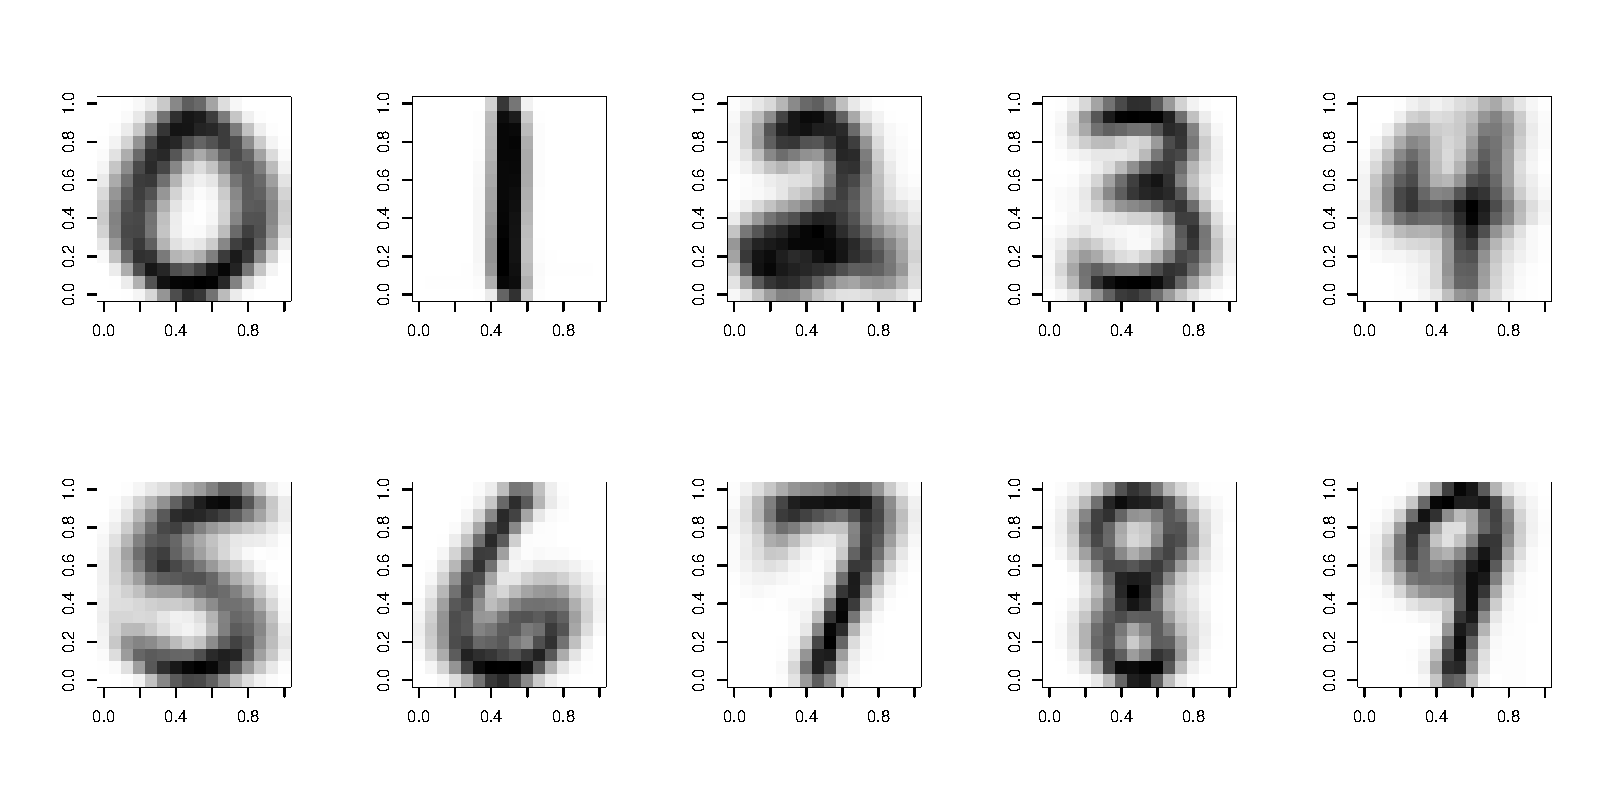
\includegraphics[width=0.8\textwidth]{image-mean}
  \caption{The mean of each digit from the training sample.}
  \label{fig:sampledigit}
\end{figure}
\end{itemize}
\end{frame}

\begin{frame}
\frametitle{The naive method}

\begin{itemize}
\item Now it is the time to check the testing sample to the mean of the training
sample. We pick the first five testing digits.

\item  We find the first, third and the fifth are rather
easy to classify by eyeballs. But the second and fourth ones are particular
difficult.
\begin{figure}
  \centering
  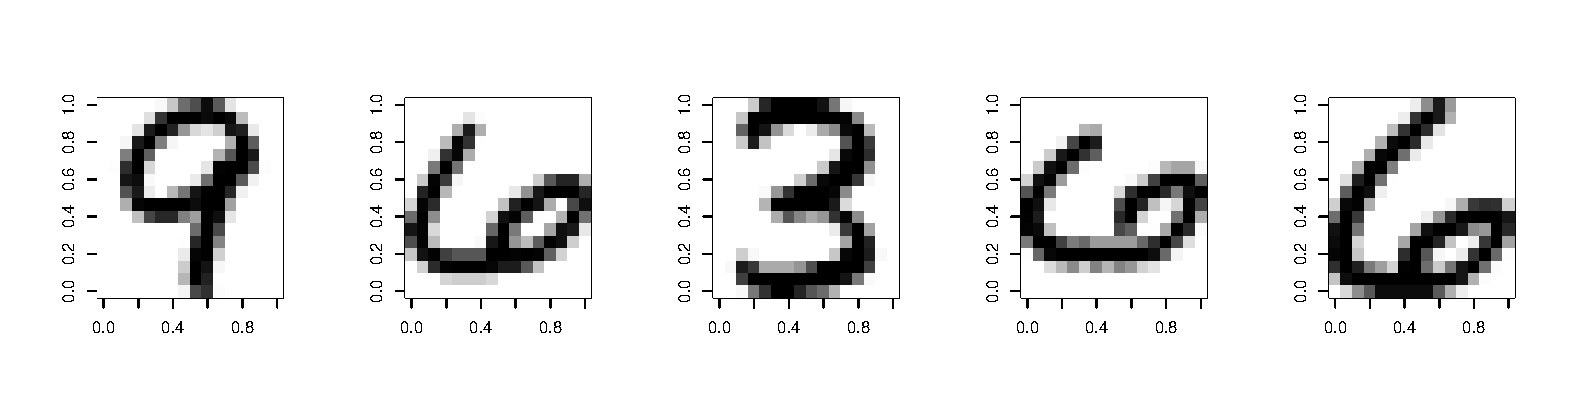
\includegraphics[width=0.7\textwidth]{test5}
  \caption{The testing image}
  \label{fig:test5}
\end{figure}

\end{itemize}
\end{frame}



\begin{frame}
\frametitle{The SVD method}

\begin{itemize}
\item We pick the digit $9$ as an example in this method and plot the first ten
singular image from the SVD decomposition

\item We first use four bases, which yields the correct specification as
  follows We also tries to classify other digits which gives robust
  results. But when we increase more basis function, there comes the risk of
  overfitting.

\item It maybe not a good idea to use all the bases but one can always pick up
  the bases according to the first $k$th largest eigen values.

\end{itemize}

\end{frame}


\begin{frame}
\frametitle{The SVD method}

\begin{figure}[h]
  \centering
 % \caption{The testing image}
  \label{fig:test9}
\end{figure}
\begin{figure}
  \centering
  \includegraphics[width=0.2\textwidth]{test9}\\
  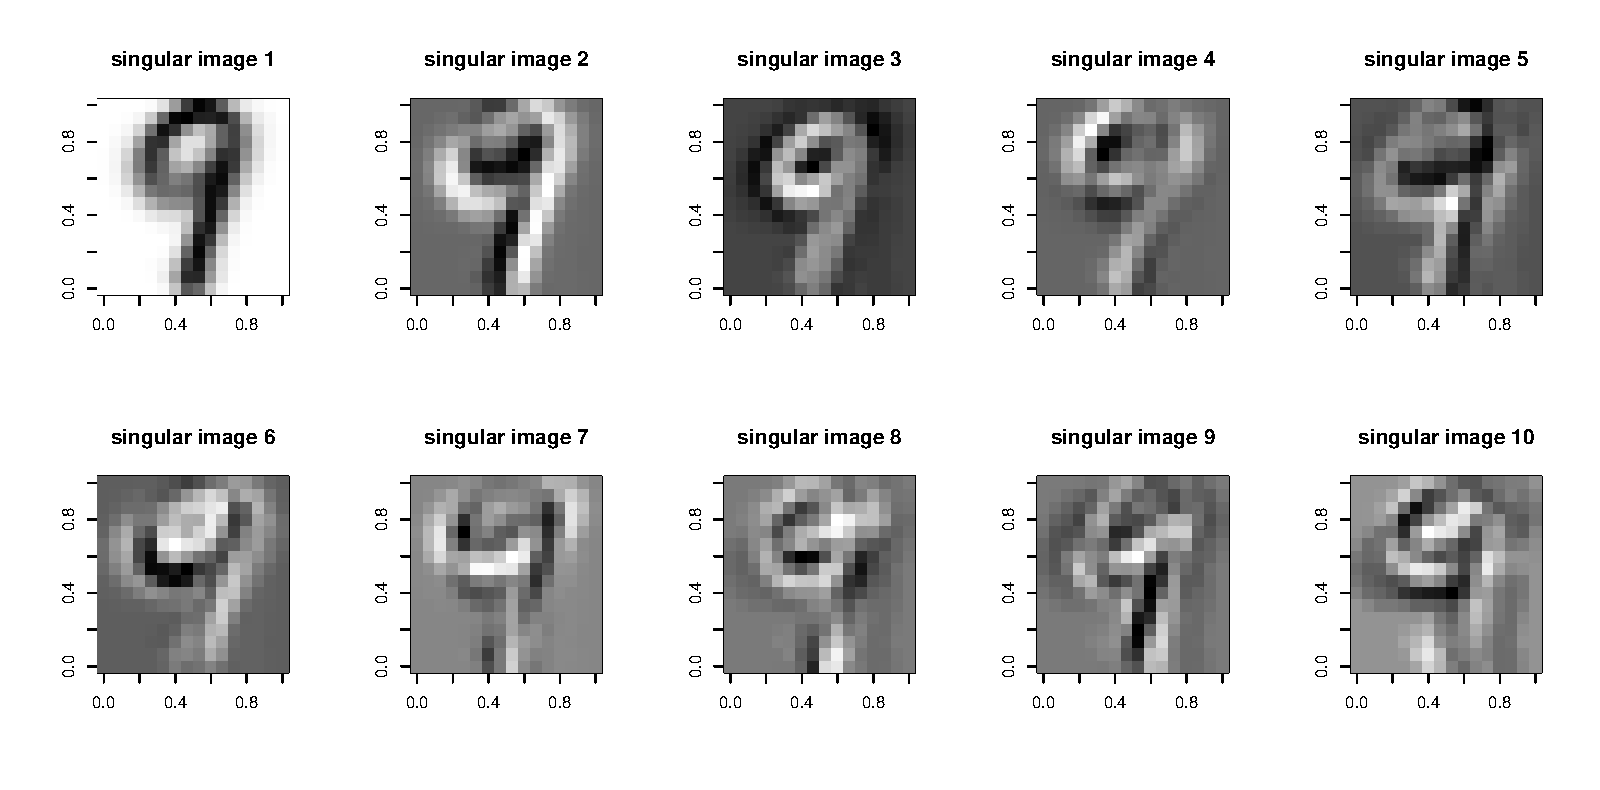
\includegraphics[width=0.7\textwidth]{singular-img-9}
  \caption{The first ten sigumar images from the training sample for digit 9.}
  \label{fig:svdimg}
\end{figure}

\end{frame}


\begin{frame}
  \frametitle{The SVD method}

  \begin{itemize}
  \item We will find out when we overfit (see the plot of classification
    success as a function of the number of basis vectors.)

  \item To see this, we loop over all testing observations and number of bases
    from 1 to 88, and then count the correct specification numbers.


\begin{figure}
  \centering
  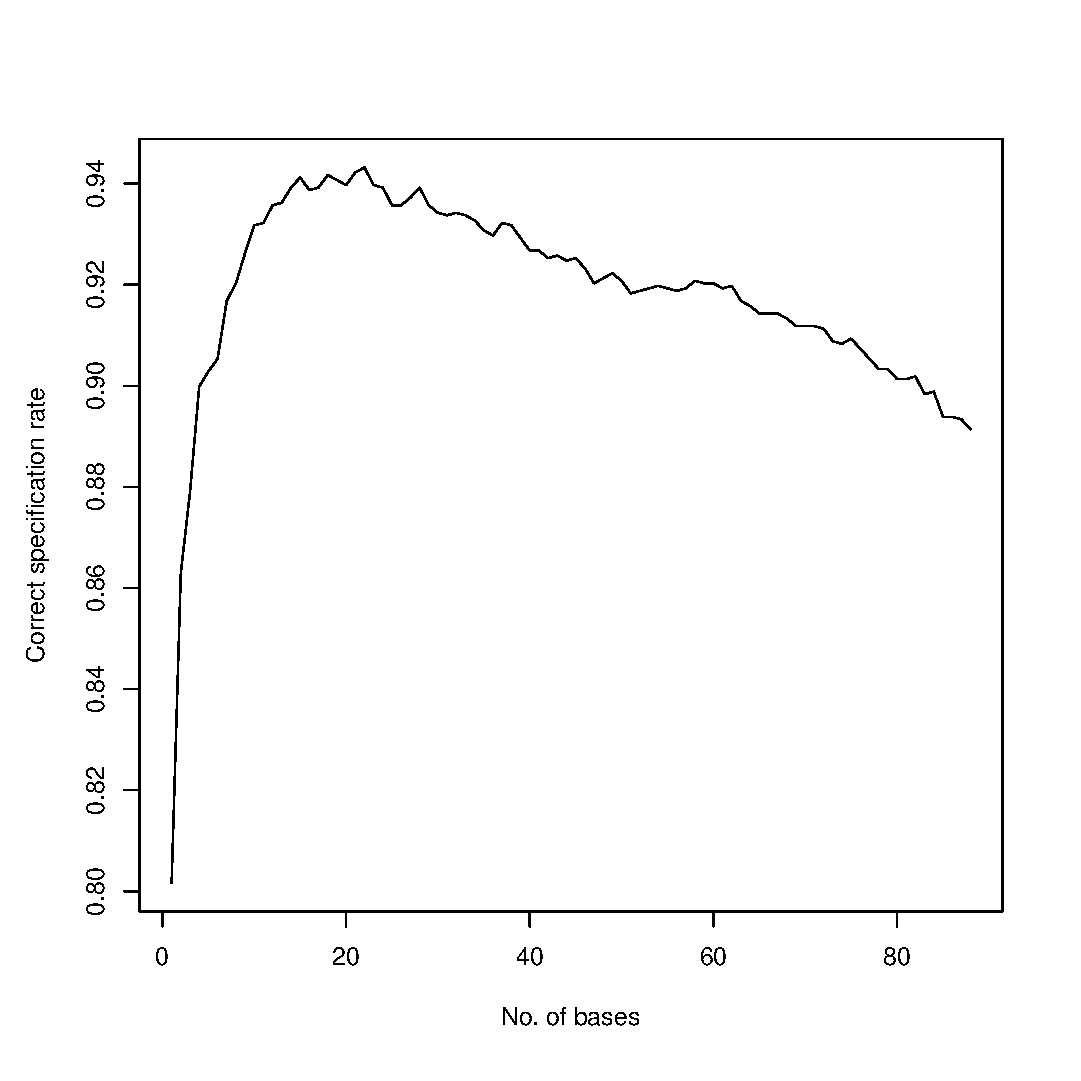
\includegraphics[width=0.55\textwidth]{CorrectSpect}
  \caption{Specification ratio with respect to the number of bases used}
  \label{fig:bases}
\end{figure}


  \end{itemize}

\end{frame}

\section{SVD in Linear Squares}

\begin{frame}
  \frametitle{Linear Regression}

  \begin{itemize}
  \item The least square solution of $y=X\beta + \epsilon$ may not be
    exist due to $X'X$ is singular.

  \item If $X'X$ is ill-conditioned or singular, we can use SVD to
    obtain a least squares solution as follows:

    \begin{equation*}
      \hat \beta = (X'X)^{-1}X'y = X^{+} y \approx V \Sigma_0^{-1} U^T y
    \end{equation*}
    where $X^{+}$ is the general inverse, and
    \begin{equation*}
      \Sigma_0^{-1} = \begin{cases}
        1/\Sigma_{ii} & \Sigma_{ii} > \epsilon\\
        0, & Otherwise\\
      \end{cases}
    \end{equation*}

  \end{itemize}


\end{frame}

\begin{frame}
  % I've seen it claimed that the solution to the minimization
  % problem $$\underset{\textbf{b}}{\text{argmin}} \ ||\textbf{A}
  % \textbf{b}|$$ subject to a constraint $||\textbf{b}||=1$, is given
  % by first finding the singular value decomposition of
  % A, $$\textbf{A} = \bf{U \Sigma V}$$ And then taking the column of
  % $\bf{V}$ corresponding to the smallest singular value. $$\ $$ Can
  % someone present a proof that this is so?
  % Norm $\| \cdot \|$ is invariant under unitary transformation so:
  % $$\|Ab\| =\| U\Sigma V^* b\| = \|\Sigma b'\|$$
  % Where $b' = V^* b$, so $\|b'\| = \|V^* b\| = \|b\| = 1$.  Next we
  % have that:
  % $$\text{argmin}_b \|\Sigma V^* b\| = V\text{argmin}_{b'} \| \Sigma b' \|$$
  % This is because $V^*$ maps unit sphere onto unit sphere.  And that
  % $b'$ which minimizes $\|\Sigma b'\|$ is $(0,\dots,0,1)^T$.
  % Finally
  % $V (0,\dots,0,1)^T$ is equal to the last column of $V$.

\end{frame}


% \begin{frame}
%   \frametitle{Suggested Reading}

%   \begin{itemize}
%   \item Jones (2009), \textbf{Chapter 3.7, 5.6, 8.3, 9.3, 9.5}


%   % \emph{Monte Carlo Statistical Methods} Book by Christian P Robert and George
%   % Casella. (2004 edition)

%   \end{itemize}

% \end{frame}

\end{document}
